\documentclass{standalone}
\usepackage{tikz,pgfplots,calc,tkz-euclide}
\usetikzlibrary{positioning,calc}
\usetikzlibrary{arrows}
\usepackage{tkz-euclide}
\usetkzobj{all}

\usepackage{xcolor}
% \definecolor{myblue}{RGB}{0, 100, 220}
\definecolor{myblue}{RGB}{0, 0, 0}

\tikzstyle{densely dashed}=          [dash pattern=on 3pt off 1pt]

\begin{document}
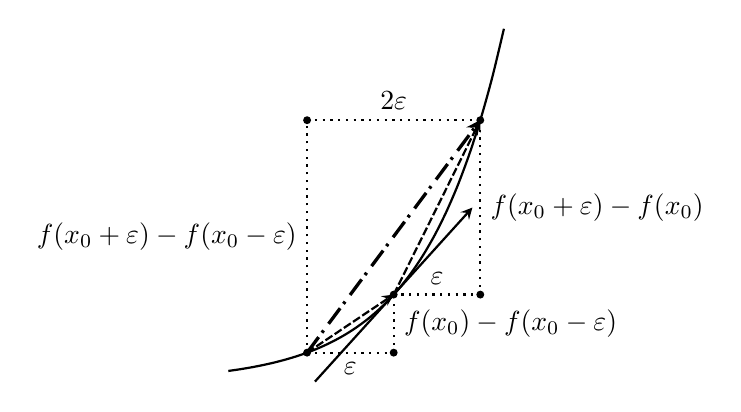
\begin{tikzpicture}[>=stealth, thick]
    \def\a{1}
    \draw[domain=-2:1.5,smooth,variable=\x,black] plot ({\x},{exp(\a*\x)});      
    \foreach \xx in {.1}{
        \draw[->, black, thick, domain=(\xx-1):(\xx+1),smooth,variable=\x] plot ({\x},{(\a*exp(\a*\xx))*(\x - \xx) + exp(\a*\xx)});      
    }

    \def\x{.1}
    \def\xp{1.2}
    \def\xm{-1}
    \def\y{{exp(\a*\x)}}
    \def\yp{{exp(\a*\xp)}}
    \def\ym{{exp(\a*\xm)}}

    \draw [->, black, densely dashed] (\xm, \ym)  --  (\x, \y);
    \draw [->, black, densely dashed] (\x, \y)  --  (\xp, \yp);
    \draw [->, myblue, dash pattern={on 7pt off 2pt on 1pt off 3pt}, very thick] (\xm, \ym)  --  (\xp, \yp);

    \draw [dotted] (\xm, \ym)  --  node[below] {$\varepsilon$} (\x, \ym);
    \draw [dotted] (\x, \y)  --  node[above] {$\varepsilon$} (\xp, \y);
    \draw [dotted] (\x, \ym)  --  node[right]{$f(x_0) - f(x_0 - \varepsilon)$} (\x, \y);
    \draw [dotted] (\xp, \y)  --  node[right]{$f(x_0 + \varepsilon) - f(x_0)$} (\xp, \yp);


    \draw [dotted] (\xm, \ym)  --  node[left]{$f(x_0 + \varepsilon) - f(x_0 - \varepsilon)$} (\xm, \yp);
    \draw [dotted] (\xm, \yp)  --  node[above]{$2\varepsilon$} (\xp, \yp);

    \draw [fill = black, draw = black] (\x, \y ) circle (1pt);
    \draw [fill = black, draw = black] (\xp, \yp) circle (1pt);
    \draw [fill = black, draw = black] (\xm, \ym) circle (1pt);
    \draw [fill = black, draw = black] (\x, \ym) circle (1pt);
    \draw [fill = black, draw = black] (\xm, \yp) circle (1pt);
    \draw [fill = black, draw = black] (\xp, \y) circle (1pt);

\end{tikzpicture}
\end{document}